\clearpage\section{Chapter 10: Inheritance and Associations}

Relationships between classes are depicted in UML class diagrams by
lines drawn between two or more class rectangles. One of the most
important relationships between classes describes the situation when
one class is an extension or minor variation of another class: this is
called generalization, or \textit{inheritance}. Most other
relationships between classes are really relationships between those
classes{\textquotesingle} \index{instance}instances at run-time; these
relationships are called \textit{associations}. This chapter starts
with inheritance, and then describes a variety of associations. \ In
this chapter you will learn how to:

\begin{itemize}
\item Define a new class in terms of its differences from an existing
class
\item Compose aggregate classes from component parts.
\item Specify new kinds of associations
\item Supply details about the roles and number of objects in an
association
\item Use structure types from Chapter 2 to implement associations
\end{itemize}

\subsection{Inheritance}

In many cases, several classes of objects are very similar. In
particular, many classes arise as enhancements of classes that have
already been defined. Enhancements might consist of added fields, added
methods, or both. In other cases a class is just a special case of
another class. For example, if you have a class
\textsf{fraction(numerator, denominator)}, you could define class
\textsf{inverses(denominator)} whose behavior is identical to that of a
fraction, but whose numerator is always 1. 

Both of these ideas are realized with the concept of
\index{inheritance}inheritance. When the definition of a class is best
expressed in terms of the definition of another class or classes, we
call that class a \index{subclass}\textit{subclass.} The class or
classes from which a subclass obtains its definition are called
\index{superclass}\textit{superclass}\textit{es}. The logical relation
between the subclass and superclass is called \textit{hyponymy}. It
means an object of the subclass can be manipulated just as if it were
an object of one of its defining classes. In practical terms it means
that similar objects can share the code that manipulates their fields.

Inheritance appears in a class diagram as a line between classes with an
arrow at one end. The arrow points to the superclass, the source of
behavior inherited by the other class. Consider Figure 10-1, in which
an offer of a salaried appointment is defined as one kind of job offer.
The attributes (\textsf{salary}, \textsf{title}) and methods
(\textsf{Accept()} and \textsf{Reject()}) of class JobOffer are
inherited by class SalariedAppointment, and do not need to be repeated
there. A new attribute (term) is added in \textsf{SalariedAppointment}
that is not in \textsf{JobOffer}.

\bigskip

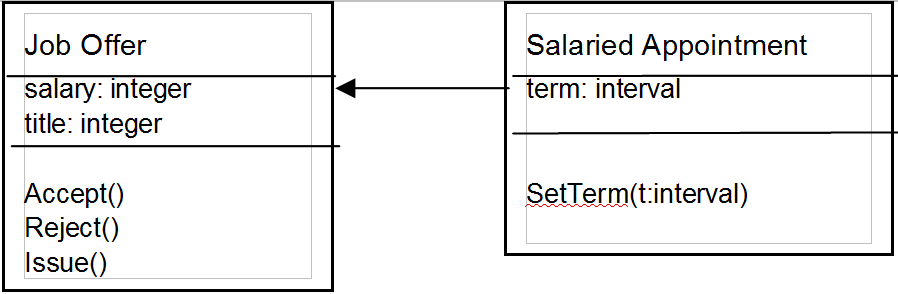
\includegraphics[width=4.9in,height=1.9in]{ub-img/subclass.png} 

{\sffamily\bfseries Figure 10-1:}
{\sffamily A Salaried Appointment is a subclass of a Job Offer}

\bigskip

The syntax of a subclass is 

\iconcode{
class \textit{classname} \textit{superclasses} (\textit{attributes}) \\
\>   \textit{methods} \\
{\sffamily\itshape
initially\_section} \\
end
}

Where \textsf{\textit{superclasses}} is an optional list of class names
separated by colons, \textsf{\textit{attributes}} is an optional list
of \index{variable}variable names separated by commas,
\textsf{\textit{methods}} is an optional list of declarations for the
class methods, and the \textsf{\textit{initially\_section}} is optional
initialization code for the class \index{constructor}constructor. \ For
example

\iconcode{
class SalariedAppointment : JobOffer (term) \\
\>   method SetTerm(t : interval) \\
\>   \ \ \ term := t \\
\>   end \\
initially \\
\>   /term := {\textquotedbl}unknown term{\textquotedbl} \\
end
}

As you can see, a subclass declaration is identical to a regular class,
with the addition of one or more superclass names, separated by colons.
The meaning of this declaration is the subject of the next section. 

\subsubsection[Inheritance Semantics]{Inheritance Semantics}

\index{inheritance!semantics}There are times when a new class might best
be described as a combination of two or more classes. Unicon classes
may have more than one superclass, separated by colons in the class
declaration. This is called multiple inheritance.

Subclasses define a record type consisting of all the field names of the
subclass itself and all its superclasses. The subclass has associated
methods consisting of those in its own body, those in the first
superclass that were not defined in the subclass, those in the second
superclass not defined in the subclass or the first superclass, and so
on. In ordinary single-inheritance, this addition of fields and methods
follows a simple linear bottom-up examination of each superclass,
followed in turn by its parent superclass. 

When a class has two or more superclasses, the search generalizes from a
linear sequence to an arbitrary \index{tree}tree, directed acyclic
\index{graph}graph, or full graph traversal. In Unicon,
\index{inheritance!multiple}multiple inheritance adds fields and
methods in an order defined by a depth-first traversal of the parent
edges of the superclass graph. This is discussed in more detail later
on. For now, think of the second and following superclasses in the
multiple inheritance case as adding methods and fields only if the
single-inheritance case (following the first superclass and all its
parents) has not already added a field or method of the same name. 

{\sffamily\bfseries
Warning}

{\sffamily
Care should be taken employing multiple inheritance if the two parent
classes have any fields or methods of the same name! }

Fields are initialized either by parameters to the constructor or by the
class initially section. Initially sections are methods and are
inherited in the normal way. \ It is common for a subclass initially
section to call one or more of their superclasses{\textquotesingle}
initially sections, for example:

\iconcode{
class sub : A : B(x) \\
initially \\
\>   x := 0 \\
\>   A.initially() \\
\>   B.initially() \\
end
}

It is common to have some attributes initialized by parameters, and
others within the initially section. For example, to define a class of
inverse values (numbers of the form \ \ \ \ 1 / \textit{n} where
\textit{n} is an integer) in terms of a class fraction(numerator,
denominator) one would write: 

\iconcode{
class inverse : fraction (denominator) \\
initially \\
\>   numerator := 1 \\
end
}

Objects of class inverse can be manipulated using all the methods
defined in class fraction; the code is actually shared by both classes
at runtime. 

Viewing inheritance as the addition of superclass elements not found in
the subclass is the opposite of the more traditional object-oriented
view that a subclass is an \index{instance!superclass}instance of the
superclass as augmented in the subclass definition.
Unicon{\textquotesingle}s viewpoint adds quite a bit of leverage, such
as the ability to define classes that are subclasses of each other.
This feature is described further below. 

\subsubsection[Invoking Superclass Operations]{Invoking Superclass
Operations}

\index{superclass!operations}When a \index{subclass}subclass defines a
method of the same name as a method defined in the superclass,
invocations on subclass objects always result in the
subclass{\textquotesingle} version of the
\index{method!overriding}method. This can be overridden by explicitly
including the superclass name in the invocation: 

\iconcode{
\>   object\$superclass.method(parameters)}

This facility allows the subclass method to do any additional work
required for added fields before or after calling an appropriate
superclass method to achieve inherited behavior. The result is
frequently a chain of inherited method invocations. 

Since initially sections are methods, they can invoke superclass
operations including superclass initially sections. This allows a chain
of initially sections to be specified to execute in either
subclass-first or superclass-first order, or some mixture of the two. 

\subsubsection[Inheritance Examples]{Inheritance Examples}

Several examples of inheritance can be obtained by extending the buffer
example from the previous chapter. Suppose the application is more than
a text \index{editor}editor: it includes word-associative databases
such as a dictionary, bibliography, spell-checker, and thesaurus. These
various databases can be represented internally using the table type.
The entries for the databases vary, but the databases all use a string
keyword lookup. As external data, the databases can be stored in text
files, one entry per line, with the keyword at the beginning. The
format of the rest of the line varies from database to database.

Figure 10-2 shows a class diagram with several subclasses derived from
class \textsf{buffer}. A class named \textsf{buftable} refines the
buffer class, adding support for random access. Three other classes are
defined as subclasses of \textsf{buftable}. The implementation of these
classes is given below.


\begin{center}
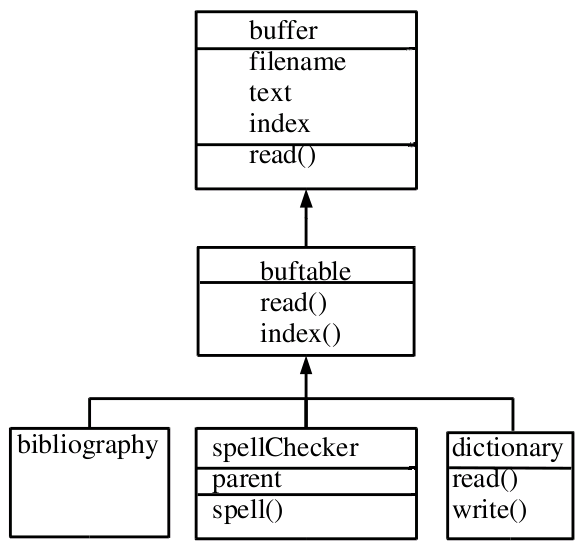
\includegraphics[width=4in,height=3.7in]{ub-img/ub-img43.png}
\end{center}

{\sffamily\bfseries Figure 10-2:}
{\sffamily Some Subclasses of the Buffer Class}

\bigskip

Although all these types of data are different, the code used to read
the data files can be shared, as well as the initial construction of
the tables. In fact, since we are storing our data one entry per line
in text files, we can use the code already written for buffers to do
the file I/O itself. 

\iconcode{
class buftable : buffer() \\
\ \ method read() \\
\>   \ self.buffer.read() \\
\>   \ tmp := table() \\
\>   \ every line := !text do \\
\>   \ \ \ line ? \{ tmp[tab(many(\&letters))] := line {\textbar} fail
\} \\
\>   \ text := tmp \\
\>   \ return \\
\ \ end \\
\ \ method index(s) \\
\>   \ return text[s] \\
\ \ end \\
end
}

This concise example shows how little must be written to achieve data
structures with vastly different behavioral characteristics, by
building on code that is already written. The superclass
\textsf{read()} operation is one important step of the subclass
\textsf{read()} operation. This technique is common enough to have a
name: it is called \textit{method
}\index{method!combination}\textit{combination} in the literature. It
allows you to view the subclass as a transformation of the superclass.
The \textsf{buftable} class is given in its entirety, but our code
sharing example is not complete: what about the data structures
required to support the databases themselves? They are all variants of
the \textsf{buftable} class, and a set of possible implementations
follow. Note that the formats presented are designed to illustrate code
sharing; clearly, an actual application might make different choices. 

\paragraph{Bibliographies}
Bibliographies might consist of a keyword followed by an uninterpreted
string of information. This imposes no additional structure on the data
beyond that imposed by the \textsf{buftable} class. An example keyword
would be Jeffery99. 

\iconcode{
class bibliography : buftable() \\
end
}

\paragraph{Spell-checkers}
The database for a spell-checker might be just a list of words, one per
line, the minimal structure required by the \textsf{buftable} class
given above. Some classes exist to introduce new terminology rather
than to define a new data structure. In this case we introduce a lookup
operation that can fail, for use in tests. In addition, since many
spell-checking systems allow user definable dictionaries in addition to
their central database, we allow \textsf{spellChecker} objects to chain
together for the purpose of looking up words. 

\iconcode{
class spellChecker : buftable(parent) \\
\ \ method spell(s) \\
\>   \ return {\textbackslash}text[s] {\textbar}
({\textbackslash}parent).spell(s) \\
\ \ end \\
end
}

\paragraph{Dictionaries}
Dictionaries are slightly more involved. Each entry might consist of a
part of speech, an etymology, and an arbitrary string of uninterpreted
text comprising a definition for that entry, separated by semicolons.
Since each such entry is itself a structure, a sensible decomposition
of the dictionary structure consists of two classes: one that manages
the table and external file I/O, and one that handles the manipulation
of dictionary entries, including their decoding and encoding as
strings. 

\iconcode{
class dictionaryentry(word, partofspeech, etymology, definition) \\
\ \ \# decode a dictionary entry into its components \\
\ \ method decode(s)  \\
\>   \ s ? \{ \\
\>   \ \ \ word \ \ \ \ \ \ \ \ :=
tab(upto({\textquotesingle};{\textquotesingle})) \\
\>   \ \ \ move(1) \\
\>   \ \ \ partofspeech :=
tab(upto({\textquotesingle};{\textquotesingle})) \\
\>   \ \ \ move(1) \\
\>   \ \ \ etymology \ \ \ :=
tab(upto({\textquotesingle};{\textquotesingle})) \\
\>   \ \ \ move(1) \\
\>   \ \ \ definition \ \ := tab(0) \\
\>   \ \} \\
\ \ end \\
\ \ method encode() \ \# encode a dictionary entry into a string \\
\>   \ return word {\textbar}{\textbar} {\textquotedbl};{\textquotedbl}
{\textbar}{\textbar} partofspeech {\textbar}{\textbar}
{\textquotedbl};{\textquotedbl} {\textbar}{\textbar} \\
\>   \ \ \ \ \ \ \ \ \ \ etymology {\textbar}{\textbar}
{\textquotedbl};{\textquotedbl} {\textbar}{\textbar} definition \\
\ \ end \\
initially \\
\ \ if /partofspeech then \{ \\
\>   \ \# constructor was called with a single string argument \\
\>   \ decode(word) \\
\>   \ \} \\
end \\
\ \\
class dictionary : buftable() \\
\ \ method read() \\
\>   \ self.buffer.read() \\
\>   \ tmp := table() \\
\>   \ every line := !text do \\
\>   \ \ \ line ? \{ \\
\>   \ \ \ \ \ tmp[tab(many(\&letters))] := dictionaryentry(line)
{\textbar} fail \\
\>   \ \ \ \ \ \} \\
\>   \ text := tmp \\
\ \ end \\
\ \ method write() \\
\>   \ f := open(filename, {\textquotedbl}w{\textquotedbl}) {\textbar}
fail \\
\>   \ every write(f, (!text).encode) \\
\>   \ close(f) \\
\ \ end \\
end
}

\paragraph{Thesauri}
Although an oversimplification, one might conceive of a thesaurus as a
list of entries, each of which consists of a comma-separated list of
synonyms followed by a comma-separated list of antonyms, with a
semicolon separating the two lists. Since the code for such a structure
is nearly identical to that given for dictionaries above, we omit it
here (you might start by generalizing class \textsf{dictionaryentry} to
handle arbitrary strings organized as fields separated by semicolons). 

\subsubsection{Superclass Cycles and Type Equivalence}
In many situations, there are several ways to represent the same
abstract type. Two-dimensional points might be represented by
\index{Cartesian coordinates}Cartesian coordinates x and y, or
equivalently by radial coordinates expressed as a distance d and angle
r given in \index{radian}radians. If one implements classes
corresponding to these types there is no reason one of them should be
considered a subclass of the other; they are interchangeable and
equivalent. 

In Unicon, expressing this equivalence is simple and direct. In defining
classes \textsf{Cartesian} and \textsf{Radial} we may declare them to
be superclasses of each other: 

\iconcode{
class Cartesian : Radial (x, y) \\
\# code that manipulates objects using Cartesian coordinates \\
end \\
\ \\
class Radial : Cartesian (d, r) \\
\# code that manipulates objects using \index{radial coordinates}radial
coordinates \\
end
}

These superclass declarations make the two types equivalent names for
the same type of object; after inheritance,
\index{instance!class}\index{instance}instances of both classes will
have fields x, y, d, and r, and support the same set of operations. 

Equivalent types each have a unique \index{constructor!class}constructor
given by their class name. Often the differing order of the parameters
used in equivalent types{\textquotesingle} constructors reflects
different points of view. Although they export the same set of
operations, the actual procedures invoked by equivalent
types{\textquotesingle} instances may be different. For example, if
both classes define an implementation of a method \textsf{print()}, the
method invoked by a given instance depends on which constructor was
used when the object was created.

If a class inherits any methods from one of its equivalent classes, it
is responsible for initializing the state of all the fields used by
those methods in its own constructor. It is also responsible for
maintaining the state of the inherited fields when its methods make
state changes to its own fields. In the geometric example given above,
for class \textsf{Radial} to use any methods inherited from class
\textsf{Cartesian}, it must at least initialize \textsf{x} and
\textsf{y} explicitly in its constructor from calculations on its
\textsf{d} and \textsf{r} parameters. In general, this added
responsibility is minimized in those classes that treat an
object{\textquotesingle}s state as immutable.

\subsection{Associations}
An \index{association}association denotes a relationship between classes
that occurs between particular instances of those classes at runtime.
In the same sense that objects are instances of classes, associations
have instances called \index{link!association instance}\textit{links.}
Like objects, links have a limited lifetime, starting from the instant
at which the relationship is established to the time at which the
relationship is dissolved. Besides serving to connect two objects,
links may have additional state information or behavior; in the most
general case links can be considered to be objects themselves: special
objects whose primary role is to interconnect other objects.

\subsubsection{Aggregation}
Inheritance may be the most famous kind of relationship between classes,
but it is not the most indispensable. Many languages that provide
objects do not even bother with inheritance. The composition of
assembly objects from their component parts, on the other hand, is a
truly ubiquitous and essential idea called
\index{aggregation}\textit{aggregation}. The class \textsf{dictionary}
defined in the previous section is a good example of an aggregate
object; its component parts are \textsf{dictionaryentry} objects.

Aggregation is depicted in class diagrams by a line between classes with
a diamond marking the aggregate, or assembly, class. \ Figure 10-3
shows an aggregate found in the domain of sports, where a team is
comprised of a group of players.

\bigskip

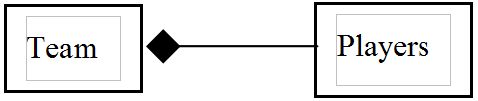
\includegraphics[width=4.0in,height=0.8in]{ub-img/aggregat.png} 

{\sffamily\bfseries Figure 10-3:}
{\sffamily A Team is an Aggregation of Players}

\bigskip

Unlike inheritance, aggregation describes a relationship between
instances at run-time. Different aggregate instances are assembled from
different component part instances. While a given player might play for
different teams over a period of time, at any given instant a player is
normally part of at most one team.

\subsubsection{User-Defined Associations}
All the other relationships between classes in \index{UML}UML are left
to the application designer to specify as custom associations.
User-defined associations are depicted by lines, annotated with the
association name next to the line, midway between the two classes.
Figure 10-4 shows a silly user-defined association that describes a
family relationship called Marriage. For a diagram containing such an
association to be well defined, the semantics of such a relationship
must be specified in external documentation that describes Marriage for
the purposes of the application at hand.

\bigskip

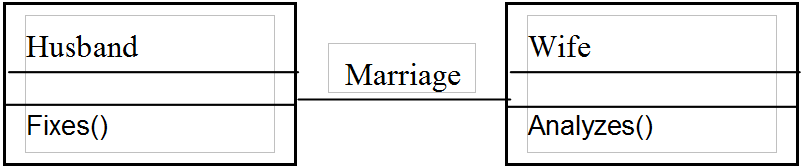
\includegraphics[width=4.8in,height=1.0in]{ub-img/marriage.png} 

{\sffamily\bfseries Figure 10-4:}
{\sffamily A User-Defined Association}

\bigskip

\subsubsection{Multiplicities, Roles, and Qualifiers}
Whether they are aggregations or user-defined application domain
relationships, associations are not completely specified until
additional details are determined during program design, such as how
many instances of each type of object may participate in a given
relationship. These additional details appear in canonical positions
relative to the line that depicts the association within a class
diagram.

A \index{multiplicity}\textit{multiplicity} is a number or range that
indicates how many instances of a class are involved in the links for
an association. In the absence of multiplicity information an
association is interpreted as involving just one instance. It normally
appears just below the association line next to the class to which it
applies. Figure 10-5 shows a BasketballTeam that is an aggregate with a
multiplicity of five Players.

\bigskip

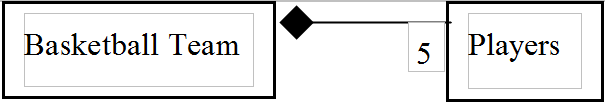
\includegraphics[width=4.8in,height=0.8in]{ub-img/multipcy.png}

{\sffamily\bfseries Figure 10-5:}
{\sffamily Multiplicity of a Basketball Team}

\bigskip

A multiplicity range is expressed as a pair of numbers separated by two
periods, as in 1..3. The value * may be used by itself to indicate that
a link may associate any number (zero or more) of objects. The * value
may also be used in a range expression to indicate no upper bound is
present, as in the range 2..*.

A \index{role}\textit{role} is a name used to distinguish different
participants and responsibilities within an association. Roles are
drawn just above or below the association line, adjacent to the class
to which they refer. They are especially useful if a given association
may link multiple instances of the same class in asymmetric
relationships. Figure 10-6 shows a better model of the classes and
roles involved in a Marriage association depicted earlier in Figure
10-4.

\bigskip

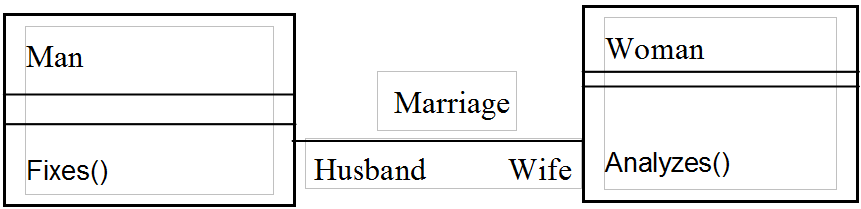
\includegraphics[width=4.8in,height=1.2in]{ub-img/roles.png}


{\sffamily\bfseries Figure 10-6:}
{\sffamily Roles in an Association}

\bigskip

A \index{qualifier}\textit{qualifier} is a key value used to efficiently
distinguish and directly access instances in a link, in lieu of a large
multiplicity that would otherwise be inefficient. For example, a
directory may contain many files, but each one may be directly accessed
by name. A qualifier is drawn as a rectangular association end with the
qualifier key given inside the rectangle. Figure 10-7 shows a
reinterpretation of the basketball aggregation in which the players on
the team are distinguished using a qualifier key named position.


\bigskip

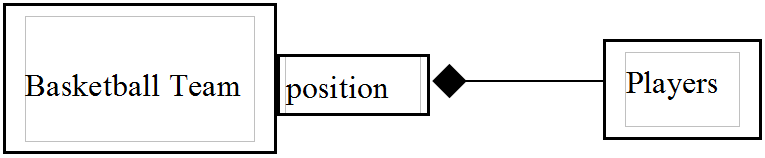
\includegraphics[width=4.8in,height=0.9in]{ub-img/qualifier.png}

{\sffamily\bfseries Figure 10-7:}
{\sffamily Using a Qualifier in Lieu of Multiplicity}

\bigskip

\subsubsection{Implementing Associations}
Unlike inheritance, which is implemented by the language and resolved at
\index{compile time}compile time, associations involve dynamic
relationships established at runtime, and are implemented by the
programmer...or are they? In the most general case, an association may
be implemented by writing a class whose instances are links between the
related classes{\textquotesingle} objects. \ In the narrowest special
case, an association can be implemented by adding an attribute in one
class to contain a \index{reference}reference to an object in an
associated class. Much of the value introduced by multiplicity and
qualifier information is to narrow the association semantics down to
what is readily implementable using the built-in structure types
instead of writing classes for them. If an association can be
implemented using a list or table instead of defining a new class, the
resulting code will be smaller and faster.

In all cases, associations will introduce additional fields into the
classes being associated. The following code example implements the
Marriage association from Figure 10-6. For illustration purposes it is
modeled as a one-one relationship at any given point in time. Notice
the intertwining methods in the two classes that establish a
bi-directional relationship. \ Error checking is left as an exercise
for the reader.

\iconcode{
class Man(wife) \\
\>   method Marry(w) \\
\>   \ \ \ wife := w \\
\>   \ \ \ if not (self === w.husband) then w.Marry(self) \\
\>   end \\
end \\
class Woman(husband) \\
\>   method Marry(m) \\
\>   \ \ \ husband := m \\
\>   \ \ \ if not (self === m.wife) then m.Marry(self) \\
\>   end \\
end
}

As a general rule, an association that has a qualifier may be
implemented using a table. The following code example corresponds to
the basketball team diagram in Figure 10-7. The players attribute might
be a list or set in class Team, but the qualifier allows class
BasketballTeam to override this and implement players using a table.
Such a refinement can be awkward in a statically typed object-oriented
language.

Depending on whether its player parameter is supplied or is null, method
\textsf{Player()} serves to either lookup a player, given a position,
or to insert a player into the association. In either case the player
at the designated position is returned.

\iconcode{
class BasketballTeam : Team () \\
\>   method Player(position, player) \\
\>   \ \ \ players[position] := {\textbackslash}player \\
\>   \ \ \ return players[position] \\
\>   end \\
initially \\
\>   players := table() \\
end
}

Associations with multiplicity might be implemented using sets or lists,
with lists being favored when multiplicity is bounded to some range, or
when there is a natural ordering among the instances. The following
version of the \textsf{BasketballTeam} class uses a list of five
elements to implement its aggregation, which occupies less space than
either a set or the table in the last example.

\iconcode{
class BasketballTeam : Team (players) \\
\>   method Player(player) \\
\>   \ \ \ if player === !players then fail \# already on the team \\
\>   \ \ \ if /!players := player then return \# added at null slot \\
\>   \ \ \ ?players := player \# kick someone else off team to add \\
\>   end \\
initially \\
\>   players := list(5) \\
end
}

Defining a new class to implement an association may be reserved for
rare cases such as many-many relationships and associations that have
their own state or behavior. Extended examples of associations and
their implementation are given in Part 3 of this book.

{\sffamily
Summary}

The relationships between classes are essential aspects of the
application domain that are modeled in object-oriented programs. You
can think of them as the {\textquotedbl}glue{\textquotedbl} that
connects ideas in a piece of software. Class diagrams allow many
details of such relationships to be specified graphically during
design. Unicon{\textquotesingle}s structure types allow most
associations to map very naturally onto code.

\clearpage
\bigskip
